\documentclass[aspectratio=169]{beamer}
%\documentclass[aspectratio=43]{beamer}

\usepackage{graphicx}  % Required for including images
\usepackage{natbib}
\usepackage{booktabs} % Top and bottom rules for tables
\usepackage{amssymb,amsthm,amsmath}
\usepackage{exscale}
\usepackage{natbib}
\usepackage{tikz}
\usepackage{listings}
\usepackage{color}
\usepackage{bm}
% Setup TikZ
\usepackage{tikz}
\usetikzlibrary{arrows}
\tikzstyle{block}=[draw opacity=0.7,line width=1.4cm]
% Setup hyperref
\usepackage{hyperref}
\hypersetup{colorlinks=true}
\hypersetup{citecolor=porange}
\hypersetup{urlcolor=porange!80!}
\hypersetup{linkcolor=porange}

\newtheorem{proposition}{Proposition}
\newtheorem{remark}{Remark}
\newtheorem{principle}{Principle}

%% Writing quarters
\newcommand{\wQ}[1]{{\textcolor{white}{Q#1}}}
\newcommand{\bQ}[1]{{Q#1}}

% Uncomment appropriate command to disable/enable hiding
%\newcommand{\mypause}{\pause}
\newcommand{\mypause}{}

\DeclareMathAlphabet{\mathpzc}{OT1}{pzc}{m}{it}

%% Autoscaled figures
\newcommand{\incfig}{\centering\includegraphics}
\setkeys{Gin}{width=0.9\linewidth,keepaspectratio}

%Make the items smaller
\newcommand{\cramplist}{
	\setlength{\itemsep}{0in}
	\setlength{\partopsep}{0in}
	\setlength{\topsep}{0in}}
\newcommand{\cramp}{\setlength{\parskip}{.5\parskip}}
\newcommand{\zapspace}{\topsep=0pt\partopsep=0pt\itemsep=0pt\parskip=0pt}

\newcommand{\backupbegin}{
   \newcounter{finalframe}
   \setcounter{finalframe}{\value{framenumber}}
}
\newcommand{\backupend}{
   \setcounter{framenumber}{\value{finalframe}}
}

\usetheme[bullet=circle,% Use circles instead of squares for bullets.
          titleline=true,% Show a line below the frame title.
          ]{Princeton}

\title[{\tt }] {Lecture 13: Software and Hardware Issues in Computational Physics}%
\author[https://apc523-2020.rtfd.io]%
{Ammar H. Hakim ({\tt ahakim@pppl.gov}) \inst{1}}%

\institute[PPPL]
{ \inst{1} Princeton Plasma Physics Laboratory, Princeton, NJ %
}

\date[3/23/2020]{Princeton University, Course APC523, 2020}

\begin{document}

\begin{frame}[plain]
  \titlepage
\end{frame}

\begin{frame}{Goal: Hardware and software for Computational Physics}
  Our computation physics codes must run somewhere: Making code work
  on modern hardware and writing \emph{long-lived} and \emph{usuable}
  software is highly non-trivial task. {\bf Difficult
    and underappreciated art!}
  \mypause%
  \begin{itemize}
  \item Modern computer hardware is changing: new architectures are
    emerging (too) rapidly.
    \begin{itemize}\cramplist
    \item Pressure on hardware: make chips \emph{faster} but
      \emph{consume less energy}. Contradictory goals.
    \item New directions: many (100s or 1000s) more low-power
      ``cores'' with lower clock speed. Funded by Exascale Project in
      the US (\url{https://www.exascaleproject.org}). Aims to build
      machines that do $10^{18}$~FLOPS!
    \end{itemize}
      \mypause%
  \item Software is expensive, even (and especially) when it is free!
    \begin{itemize}\cramplist
    \item Software development is \emph{labor intensive}. Takes time,
      and humans get tired, need to sleep, eat, take vacations (and
      hide from viruses).
    \item More importantly: writing good code is an \emph{art}. Can't
      be learned only from books. Need to \emph{apprentice} yourself
      with a Master Craftsman. Process is slow, can take years to
      perfect art.
    \end{itemize}
  \end{itemize}
\end{frame}

\begin{frame}{Some History: Charles Babbage, (1791-1871)}
  \begin{columns}
    
    \begin{column}{0.4\linewidth}
      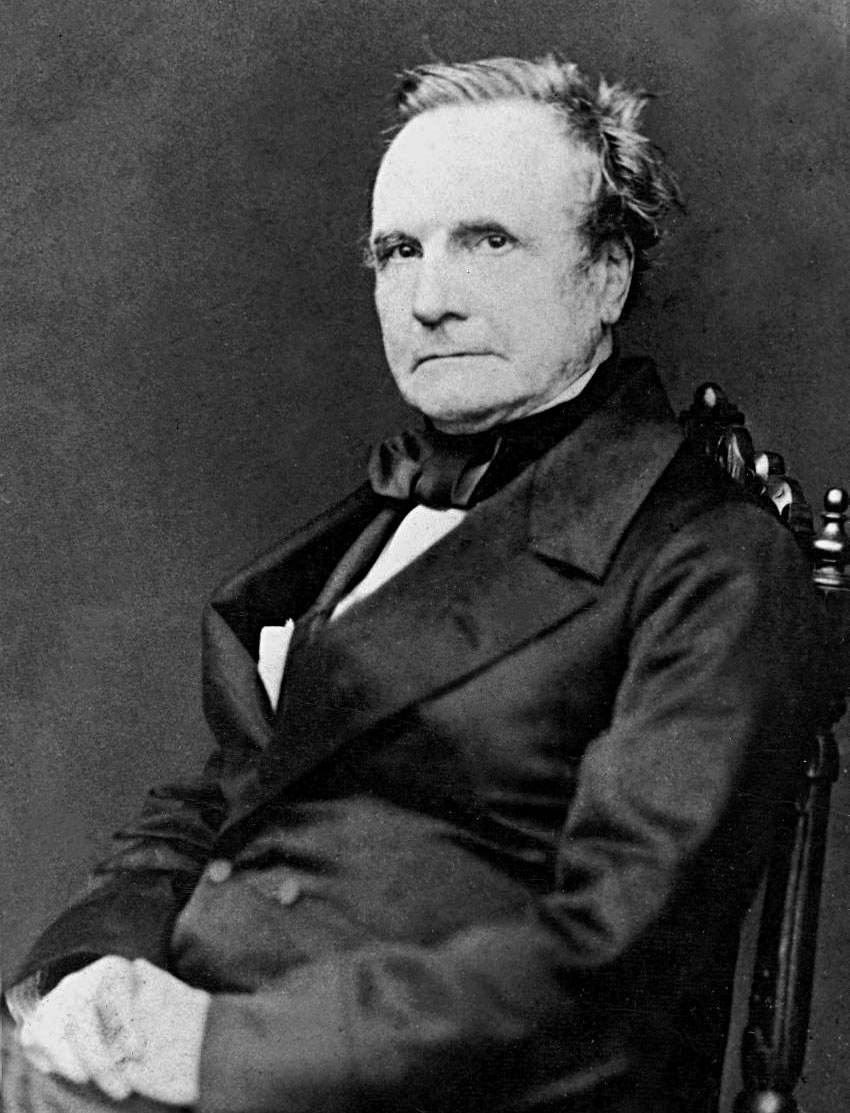
\includegraphics[width=\linewidth]{Charles_Babbage-1860.jpg}
    \end{column}

    \begin{column}{0.6\linewidth}
      \begin{itemize}\cramplist
      \item Considered to be the ``Father of the computer''. Designed
        mechanical machines to compute values of polynomial
        functions. \emph{Not completed in his lifetime}. Built by
        Science Museum, London in 1991 (printer he designed
        constructed in 2000)
        \mypause%
      \item Accomplishment of greatest genuis was the invention of the
        ``Analytical Engine''. General purpose computer, with all
        essential ideas now found in modern computer hardware worked
        out in detail.
      \end{itemize}
      See links on lecture website. See also cyberpunk novel ``The
      Difference Engine''. Explores distopian alternate history in
      which Analytical Engine built.
    \end{column}
  \end{columns}
\end{frame}

\begin{frame}{Some History: John von Neumann, (1903-1957)}
  \begin{columns}
    
    \begin{column}{0.4\linewidth}
      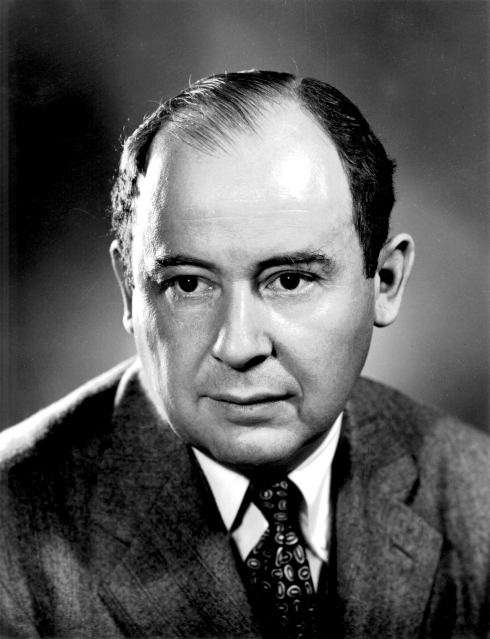
\includegraphics[width=\linewidth]{JohnvonNeumann-LosAlamos.png}
    \end{column}

    \begin{column}{0.6\linewidth}
      \begin{itemize}\cramplist
      \item Polymath of great genius: mathematician, physicist and
        computer scientist. Modern computer architecture (von Neumann
        architecture) named after him.%
        \mypause%
      \item Influential machine designed at Institute of Advanced
        Study from 1945-1951; 40-bit ``word'' with two 20-bit
        instructions; 1024 words of memory.
        \mypause%
      \item Also wrote first and highly influential paper on error
        analysis on Gaussian elimination with Herman Goldstine:
        created field of numerical analysis. See review in SIAM Rev.
        {\bf 53} (4), pp.607-682.
      \end{itemize}
    \end{column}
  \end{columns}
\end{frame}

\begin{frame}{Many others, some with Princeton background}
  The history of computing is complex and many people have played key
  role, many with Princeton backrgound (like von Neumann who was at
  IAS)
  \begin{itemize}
  \item Alan Turing. Towering genius in theoretical computer science,
    got his math Ph.D from Princeton University. Invented ``Turing
    machines'', an abstract model for universal computing
    machine. Very influential and part of modern CS curriculum. Worked
    with von Neumann on philosophy of AI and machine computability.%
    \mypause%
  \item Not so well known: Charles Sander Peirce (``Purse''). Realized
    that logical operations could be carried out by {\bf electrical
      circuits, way back in 1886}, decades before such machines were
    built! See letter in which \emph{first logic circuit} is described
    to his former student Allan Marquand of Princeton. (Science
    Library near GIS and book stacks). Rather sad letter, written when
    C.S Peirce was very poor and had to borrow money Marquand. (Art
    library named after Marquand).
  \end{itemize}
\end{frame}

\end{document}


\begin{frame}{}
\end{frame}

\begin{columns}
  
  \begin{column}{0.6\linewidth}
  \end{column}
  
  \begin{column}{0.4\linewidth}
    \includegraphics[width=\linewidth]{fig/Kinsey_2011_Pfus_vs_T.pdf}
  \end{column}
\end{columns}

% ----------------------------------------------------------------
